\documentclass[12pt]{article}

\usepackage[margin=1in]{geometry}
\usepackage[T1]{fontenc}
\usepackage{lmodern}
\usepackage{microtype}
\usepackage{amsmath,amssymb,mathtools}
\usepackage{booktabs}
\usepackage{setspace}
\usepackage{tikz}
\usepackage{hyperref}
\usepackage{xurl}

\hypersetup{
  colorlinks=true,
  linkcolor=black,
  citecolor=black,
  urlcolor=blue,
  pdftitle={The Electron's Triangle},
  pdfauthor={Light-Meter Physics},
  pdfsubject={A derivation of the relativistic energy-momentum triangle and its plane-wave consequences},
  pdfkeywords={electron, relativistic energy, momentum, Compton frequency, Klein-Gordon, Dirac}
}

\onehalfspacing
\widowpenalty=10000
\clubpenalty=10000

\title{The Electron's Triangle:\\
A Complete Derivation of the Relativistic Plane-Wave Example}
\author{Light-Meter Physics}
\date{Draft Manuscript}

\begin{document}

\maketitle

\begin{abstract}
For a free electron moving at $v=4c/5$ in one spatial dimension, the Lorentz factor is $\gamma=5/3$. The resulting total energy, momentum, and rest energy obey $E:pc:m_ec^2=5:4:3$, so the mass-shell relation becomes a $3$--$4$--$5$ right triangle. This manuscript derives that result from the free-particle proper-time action, constructs the associated positive-energy plane-wave phase, and follows the same dispersion relation into the Klein--Gordon equation. It also distinguishes laboratory velocity, wave-packet group velocity, phase velocity, and celerity; explains why the nonrelativistic kinetic-energy operator fails at this momentum without indicting quantum momentum or energy operators; and derives the Klein--Gordon current for the plane wave. The scalar Klein--Gordon calculation is used as a dispersion check, not as a complete model of an electron: electron spin requires a Dirac spinor. The phrase \emph{rest clock} is treated as a phase analogy, not as an internal clock or new physical mechanism. All results are standard relativistic and quantum-mechanical identities specialized to one transparent numerical example.
\end{abstract}

\noindent\textbf{Keywords:} relativistic energy--momentum relation, plane wave, Compton frequency, celerity, Klein--Gordon equation, Dirac spinor

\section{Introduction}

A single choice of speed makes several relativistic quantities especially simple. For a free electron moving along $+x$ with laboratory speed $v=0.8c$, the Lorentz factor is $5/3$. Its energy, momentum, and rest energy obey
\begin{equation}
  E:pc:m_ec^2=5:4:3.
\end{equation}
The invariant energy--momentum relation is therefore the familiar integer identity $5^2=4^2+3^2$, with all three sides expressed in a common energy scale $m_ec^2/3$. This is the electron's \emph{triangle} in the title.

The numerical pattern is useful because it makes several derivations easy to check: the plane-wave phase, the mass shell, the Klein--Gordon equation, and the difference between relativistic and nonrelativistic kinetic energy. It is a compact display of standard relations specialized to one selected speed. Matter-wave ideas originate with de Broglie, while Schr\"odinger's wave mechanics and the relativistic scalar equation developed in the historical work cited below \cite{deBroglie1925,Schrodinger1926,Klein1926,Gordon1926}.

The derivation keeps several concepts distinct. The ratio $\delta\tau\equiv dt/d\tau$ is dimensionless and equals $\gamma$; it is not a proper-time increment. The Lorentz-transformed coordinate $t'$ equals the electron's proper time only on its worldline. The plane wave is an ideal momentum eigenstate, not a spatially localized electron. Finally, the Klein--Gordon equation checks the relativistic dispersion relation but does not encode electron spin, which requires the Dirac theory \cite{Dirac1928}.

\section{Setup and conventions}

Work in flat spacetime with metric signature $(+,-,-,-)$ and restrict motion to the $x$ direction. The electron is free, has rest mass $m_e$, and follows an inertial trajectory with constant laboratory velocity $v>0$. Define
\begin{equation}
  \beta\equiv\frac{v}{c}=\frac{4}{5},
  \qquad
  \gamma\equiv\frac{1}{\sqrt{1-\beta^2}}=\frac{5}{3}.
  \label{eq:beta-gamma}
\end{equation}
The laboratory coordinates are $(t,x)$ and the electron's proper time along its trajectory is $\tau$. Following the Light-Meter Physics notation, set
\begin{equation}
  \delta\tau\equiv\frac{dt}{d\tau}=\gamma=\frac{5}{3}.
  \label{eq:clock-rate-ratio}
\end{equation}
Despite its typography, $\delta\tau$ in this manuscript denotes a dimensionless rate ratio, not an infinitesimal or finite time interval. The standard relation $d\tau=dt/\gamma$ follows from the invariant interval:
\begin{equation}
  c^2d\tau^2=c^2dt^2-dx^2
  =c^2dt^2(1-\beta^2),
  \qquad
  \frac{d\tau}{dt}=\sqrt{1-\beta^2}=\frac{3}{5}.
  \label{eq:proper-time}
\end{equation}

All plane-wave expressions use the positive-energy convention
\begin{equation}
  \psi(x,t)=\psi_0\exp\!\left[\frac{i}{\hbar}(px-Et)\right],
  \label{eq:phase-convention}
\end{equation}
where $\psi_0$ is a constant amplitude. The quantities $E$ and $p$ refer to total energy and laboratory momentum, respectively, unless explicitly identified as kinetic energy. The idealized plane wave extends over all space; normalization and localized wave packets are discussed later.

\section{Free-particle action, momentum, and energy}

For a free relativistic point particle, the action along a worldline segment is
\begin{equation}
  S=-m_ec^2\int d\tau.
  \label{eq:free-action}
\end{equation}
Using Eq.~\eqref{eq:proper-time}, write the same action in laboratory time:
\begin{equation}
  S=\int L(v)\,dt,
  \qquad
  L(v)=-m_ec^2\sqrt{1-\frac{v^2}{c^2}}.
  \label{eq:free-lagrangian}
\end{equation}
The canonical momentum is obtained by differentiating the Lagrangian:
\begin{align}
  p
  &=\frac{\partial L}{\partial v}
   =-m_ec^2\frac{1}{2}
     \left(1-\frac{v^2}{c^2}\right)^{-1/2}
     \left(-\frac{2v}{c^2}\right) \\
  &=\gamma m_ev.
  \label{eq:relativistic-momentum}
\end{align}
The Hamiltonian is the Legendre transform:
\begin{align}
  H&\equiv pv-L \\
   &=\gamma m_ev^2+\frac{m_ec^2}{\gamma} \\
   &=\gamma m_ec^2.
  \label{eq:relativistic-energy}
\end{align}
In the last step, $1/\gamma=\gamma(1-v^2/c^2)$ was used. For a free particle, this Hamiltonian is the total energy $E$. Thus
\begin{equation}
  E=\gamma m_ec^2,
  \qquad
  p=\gamma m_ev.
  \label{eq:E-p-general}
\end{equation}
These expressions follow from the standard relativistic point-particle action; the selected value $\beta=4/5$ is an example, not an additional dynamical postulate.

\section{From proper-time action to the plane-wave phase}

Quantum mechanics associates a phase factor $e^{iS/\hbar}$ with an action. For the free particle, Eq.~\eqref{eq:free-action} gives the phase along its worldline as
\begin{equation}
  \exp\!\left(\frac{iS}{\hbar}\right)
  =\exp\!\left(-\frac{i m_ec^2\tau}{\hbar}\right).
  \label{eq:proper-time-phase}
\end{equation}
To connect this expression to a wave over spacetime, let $S'$ be the inertial frame moving at $+v$ relative to the laboratory, in which the electron is at rest. Choose the two frame origins to coincide at $t=t'=\tau=0$. There the positive-energy plane-wave phase is $\psi'=\psi_0e^{-im_ec^2t'/\hbar}$. The Lorentz transformation is
\begin{equation}
  t'=\gamma\left(t-\frac{vx}{c^2}\right).
  \label{eq:lorentz-time}
\end{equation}
Substituting Eq.~\eqref{eq:lorentz-time} into the rest-frame phase yields
\begin{align}
  -m_ec^2t'
  &=-\gamma m_ec^2t+\gamma m_ev x \\
  &=px-Et,
  \label{eq:boosted-phase-action}
\end{align}
where Eq.~\eqref{eq:E-p-general} was used. This gives exactly the convention in Eq.~\eqref{eq:phase-convention}.

There is an important qualification: $t'$ is a Lorentz-frame coordinate at a general spacetime event, not the electron's proper time everywhere. On the electron's worldline $x=vt$, however,
\begin{equation}
  t'=\gamma t(1-\beta^2)=\frac{t}{\gamma}=\tau,
  \qquad
  px-Et=-m_ec^2\tau.
  \label{eq:phase-on-worldline}
\end{equation}
Thus the spacetime plane-wave phase agrees with the proper-time action phase along the trajectory. Calling this a \emph{rest-clock phase} is an explanatory analogy for the Compton-scale phase accumulation, not a claim that the electron contains an internal oscillator.

\section{The energy--momentum triangle}

At $\beta=4/5$, Eqs.~\eqref{eq:E-p-general} and \eqref{eq:beta-gamma} give
\begin{equation}
  E=\frac{5}{3}m_ec^2,
  \qquad
  pc=\gamma\beta m_ec^2=\frac{4}{3}m_ec^2,
  \qquad
  E:pc:m_ec^2=5:4:3.
  \label{eq:triangle-values}
\end{equation}
The general mass-shell relation follows directly:
\begin{align}
  E^2-p^2c^2
  &=\gamma^2m_e^2c^4-\gamma^2m_e^2v^2c^2 \\
  &=\gamma^2m_e^2c^4(1-\beta^2) \\
  &=m_e^2c^4.
  \label{eq:mass-shell-derivation}
\end{align}
Therefore the energy $E$ is the hypotenuse of a right triangle whose perpendicular legs are $pc$ and $m_ec^2$. Each side has units of energy. At the chosen speed,
\begin{equation}
  \left(\frac{5}{3}m_ec^2\right)^2
  =\left(\frac{4}{3}m_ec^2\right)^2+(m_ec^2)^2,
  \qquad
  5^2=4^2+3^2.
  \label{eq:345-triangle}
\end{equation}

\begin{figure}[ht]
  \centering
  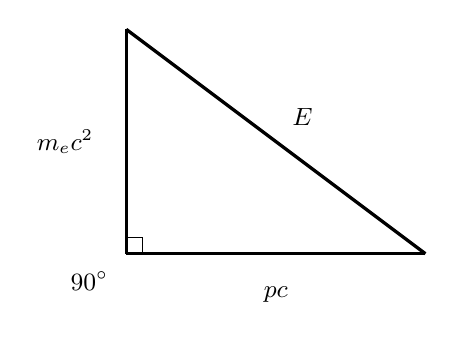
\begin{tikzpicture}[scale=0.95, every node/.style={font=\small}]
    \coordinate (O) at (0,0);
    \coordinate (A) at (0,3);
    \coordinate (B) at (4,0);
    \draw[very thick] (O)--(A) node[midway,left=8pt] {$m_ec^2$};
    \draw[very thick] (O)--(B) node[midway,below=8pt] {$pc$};
    \draw[very thick] (A)--(B) node[midway,above right=2pt] {$E$};
    \draw (0,0.22)--(0.22,0.22)--(0.22,0);
    \node[below left=3pt] at (O) {$90^\circ$};
  \end{tikzpicture}
  \caption{The mass shell drawn in the proportions $m_ec^2:pc:E=3:4:5$. The diagram is not a trajectory in physical space.}
  \label{fig:energy-triangle}
\end{figure}

The triangle also yields useful factorizations. The kinetic energy is
\begin{equation}
  K\equiv E-m_ec^2=\frac{2}{3}m_ec^2,
  \label{eq:exact-kinetic}
\end{equation}
and the two light-cone combinations obey
\begin{equation}
  E+pc=3m_ec^2,
  \qquad
  E-pc=\frac{1}{3}m_ec^2,
  \qquad
  (E+pc)(E-pc)=m_e^2c^4.
  \label{eq:light-cone-factors}
\end{equation}
The $3{:}4{:}5$ label refers only to these scaled quantities; it is not a claim that energy and momentum form an ordinary spatial triangle in the laboratory.

\section{Quantum operators and Compton scales}

For the plane wave in Eq.~\eqref{eq:phase-convention}, spatial and temporal differentiation return the phase coefficients:
\begin{align}
  \hat p_x\psi
  &\equiv-i\hbar\frac{\partial\psi}{\partial x}
   =p\psi,
  \label{eq:momentum-eigenvalue}\\
  \hat E\psi
  &\equiv i\hbar\frac{\partial\psi}{\partial t}
   =E\psi.
  \label{eq:energy-eigenvalue}
\end{align}
These are the standard momentum and energy representations on plane waves. The derivatives do not change the state except for multiplying it by its momentum or energy eigenvalue. They do not, by themselves, specify a new electron dynamics; the dispersion relation or Hamiltonian supplies that dynamics.

Define the unreduced Compton wavelength and Compton frequency by
\begin{equation}
  \lambda_C\equiv\frac{h}{m_ec},
  \qquad
  \nu_C\equiv\frac{m_ec^2}{h},
  \qquad
  T_C\equiv\frac{1}{\nu_C}=\frac{\lambda_C}{c}.
  \label{eq:compton-definitions}
\end{equation}
At $\beta=4/5$, the laboratory plane wave has
\begin{equation}
  \nu_E\equiv\frac{E}{h}=\frac{5}{3}\nu_C,
  \qquad
  \lambda=\frac{h}{p}=\frac{3}{4}\lambda_C.
  \label{eq:lab-compton-scales}
\end{equation}
The dimensionless phase angle, expressed in radians, may be written
\begin{equation}
  \psi(x,t)=\psi_0e^{i\phi(x,t)},
  \qquad
  \phi(x,t)=2\pi\nu_C\left(\frac{4x}{3c}-\frac{5t}{3}\right).
  \label{eq:phase-angle}
\end{equation}
Define positive phase rates using $-1/(2\pi)$ times the corresponding phase derivative. At a fixed laboratory position, along the electron's worldline per laboratory time, and along that worldline per proper time, respectively,
\begin{align}
  -\frac{1}{2\pi}\left.\frac{\partial\phi}{\partial t}\right|_x
  &=\nu_E=\gamma\nu_C=\frac{5}{3}\nu_C,
  \label{eq:phase-rate-fixed}\\
  -\frac{1}{2\pi}\left.\frac{d\phi}{dt}\right|_{x=vt}
  &=-\frac{1}{2\pi}\left.\left(\partial_t\phi+v\partial_x\phi\right)\right|_{x=vt}
   =\frac{\nu_C}{\gamma}=\frac{3}{5}\nu_C,
  \label{eq:phase-rate-worldline-lab}\\
  -\frac{1}{2\pi}\left.\frac{d\phi}{d\tau}\right|_{x=vt}
  &=\nu_C.
  \label{eq:phase-rate-worldline-proper}
\end{align}
These are derivatives of the same phase along different paths and with different time parameters, so the fixed-position phase frequency and the time-dilated worldline rate are compatible. They do not by themselves establish a measurable internal electron clock.

Here $\lambda_C$ is the unreduced Compton wavelength; the reduced Compton wavelength is $\hbar/(m_ec)=\lambda_C/(2\pi)$ and is not the length denoted by $\lambda_C$ in this manuscript.

Using the 2022 CODATA electron rest energy and Compton wavelength gives the illustrative values in Table~\ref{tab:numerical-values} \cite{CODATA2022}.
\begin{table}[ht]
  \centering
  \small
  \begin{tabular}{@{}lll@{}}
    \toprule
    Quantity & Exact expression at $\beta=4/5$ & Approximate value \\
    \midrule
    Rest energy & $m_ec^2$ & $0.51099895\ \mathrm{MeV}$ \\
    Total energy & $5m_ec^2/3$ & $0.85166492\ \mathrm{MeV}$ \\
    Momentum-energy & $pc=4m_ec^2/3$ & $0.68133193\ \mathrm{MeV}$ \\
    Kinetic energy & $2m_ec^2/3$ & $0.34066597\ \mathrm{MeV}$ \\
    Momentum & $4m_ec/3$ & $3.64123\times10^{-22}\ \mathrm{kg\,m\,s^{-1}}$ \\
    Compton wavelength & $h/(m_ec)$ & $2.42631\times10^{-12}\ \mathrm{m}$ \\
    Compton frequency & $\nu_C=m_ec^2/h$ & $1.23559\times10^{20}\ \mathrm{Hz}$ \\
    Laboratory phase frequency & $\nu_E=5\nu_C/3$ & $2.05932\times10^{20}\ \mathrm{Hz}$ \\
    Laboratory de Broglie wavelength & $3\lambda_C/4$ & $1.81973\times10^{-12}\ \mathrm{m}$ \\
    \bottomrule
  \end{tabular}
  \caption{Selected scales. The displayed values are rounded; the exact rational factors follow from $\beta=4/5$.}
  \label{tab:numerical-values}
\end{table}

As a separate prescribed-field scale example, the relativistic Lorentz-force approximation gives $r=p/(eB)$ for motion perpendicular to a uniform magnetic field, neglecting radiation reaction. Here $e>0$ is the magnitude of the electron charge and $p$ is its mechanical momentum. At $B=0.1\ \mathrm{T}$, $r\simeq2.273\ \mathrm{cm}$. This is a separate classical field scenario, not part of the free-plane-wave derivation.

\section{Four rates that should not be conflated}

Relativistic kinematics and the plane-wave dispersion define several distinct rates. The laboratory velocity is $v=dx/dt$. The celerity, also called proper velocity, is the spatial rate per unit particle proper time:
\begin{equation}
  u\equiv\frac{dx}{d\tau}
  =\frac{dx}{dt}\frac{dt}{d\tau}
  =\gamma v
  =\frac{p}{m_e}
  =\frac{4}{3}c.
  \label{eq:celerity}
\end{equation}
It can exceed $c$ because its denominator is the particle's proper time, not laboratory time. It is not the electron's laboratory speed.

For the plane wave, define $k\equiv p/\hbar$ and $\omega\equiv E/\hbar$.
For a positive-energy plane-wave branch with dispersion $E(p)=\sqrt{p^2c^2+m_e^2c^4}$, the phase velocity is
\begin{equation}
  v_{\mathrm{ph}}\equiv\frac{\omega}{k}=\frac{E}{p}=\frac{5}{4}c.
  \label{eq:phase-velocity}
\end{equation}
The group velocity of a narrow, freely propagating wave packet is the slope of the dispersion relation:
\begin{equation}
  v_{\mathrm{g}}\equiv\frac{d\omega}{dk}
  =\frac{dE}{dp}
  =\frac{pc^2}{E}
  =\frac{4}{5}c.
  \label{eq:group-velocity}
\end{equation}
The phase velocity may exceed $c$ without carrying a signal; it is the motion of constant-phase surfaces. The group-velocity statement applies to a sufficiently narrow free-particle packet, not to a single perfectly monochromatic plane wave. The four rates and their three distinct values are summarized in Table~\ref{tab:rates}.

\begin{table}[ht]
  \centering
  \small
  \begin{tabular}{@{}lll@{}}
    \toprule
    Rate & Definition & Value \\
    \midrule
    Laboratory velocity & $dx/dt=pc^2/E$ & $4c/5$ \\
    Group velocity & $dE/dp$ for a narrow packet & $4c/5$ \\
    Celerity & $dx/d\tau=p/m_e$ & $4c/3$ \\
    Phase velocity & $E/p$ & $5c/4$ \\
    \bottomrule
  \end{tabular}
  \caption{The laboratory velocity and narrow-packet group velocity coincide here; celerity and phase velocity have the distinct definitions shown.}
  \label{tab:rates}
\end{table}

The plane wave is an exact momentum eigenstate, corresponding to a delta-function distribution in momentum and an unlocalized position state. A physical localized state is a superposition of momenta. Its packet center moves approximately at $v_{\mathrm g}$ when the momentum spread is narrow enough that the dispersion relation is locally linear.

\section{Why the nonrelativistic Hamiltonian fails}

The momentum operator in Eq.~\eqref{eq:momentum-eigenvalue} remains the correct momentum operator. The issue is instead the use of the low-speed Hamiltonian
\begin{equation}
  \hat H_{\mathrm{NR}}=\frac{\hat p_x^2}{2m_e}
  =-\frac{\hbar^2}{2m_e}\frac{\partial^2}{\partial x^2}.
  \label{eq:nonrel-hamiltonian}
\end{equation}
At $p=4m_ec/3$, this Hamiltonian gives
\begin{equation}
  K_{\mathrm{NR}}=\frac{p^2}{2m_e}=\frac{8}{9}m_ec^2,
  \label{eq:nonrel-kinetic}
\end{equation}
whereas the exact relativistic kinetic energy from Eq.~\eqref{eq:exact-kinetic} is
\begin{equation}
  K_{\mathrm{rel}}=E-m_ec^2=\frac{2}{3}m_ec^2.
  \label{eq:rel-kinetic-again}
\end{equation}
Thus $K_{\mathrm{NR}}/K_{\mathrm{rel}}=4/3$. The nonrelativistic estimate is one third larger than the exact value at this momentum. This is expected: its expansion
\begin{equation}
  K_{\mathrm{rel}}(p)
  =\sqrt{m_e^2c^4+p^2c^2}-m_ec^2
  =\frac{p^2}{2m_e}-\frac{p^4}{8m_e^3c^2}+\cdots
  \label{eq:kinetic-expansion}
\end{equation}
is controlled only when $p\ll m_ec$, a condition not met by $p=4m_ec/3$. More precisely, the Taylor series about $p=0$ has radius of convergence $m_ec$, set by the complex branch points $p=\pm i m_ec$. The selected momentum lies outside that radius, so adding further terms of this same series does not yield a convergent repair.

It is also important to compare like with like. Acting on the total-energy phase, $i\hbar\partial_t$ returns $E$, which includes rest energy. The nonrelativistic operator $\hat H_{\mathrm{NR}}$ returns the approximate kinetic energy. If the rest-energy phase is removed by writing $\psi=e^{-im_ec^2t/\hbar}\varphi$, then the exact equation for this plane wave is $i\hbar\partial_t\varphi=K_{\mathrm{rel}}\varphi$, which still differs from $\hat H_{\mathrm{NR}}\varphi=K_{\mathrm{NR}}\varphi$. Removing a phase does not repair the low-speed approximation.

The exact relativistic Hamiltonian dispersion is $H(p)=\sqrt{p^2c^2+m_e^2c^4}$, whose group slope is $dE/dp=v$. In a first-order time-evolution equation one can use a relativistic Hamiltonian; Dirac theory supplies a local first-order wave equation for spin-$1/2$ electrons. The mismatch above is therefore a failure of the approximation $p^2/(2m_e)$ at relativistic momentum, not a failure of quantum operators or of the general equation $i\hbar\partial_t\psi=\hat H\psi$.

\section{Klein--Gordon equation as a mass-shell check}

The relativistic mass shell can be promoted to a wave equation using the energy and momentum operators:
\begin{equation}
  \left(\hat E^2-c^2\hat p_x^2-m_e^2c^4\right)\psi=0.
  \label{eq:mass-shell-operator}
\end{equation}
Substituting $\hat E=i\hbar\partial_t$ and $\hat p_x=-i\hbar\partial_x$ gives
\begin{equation}
  \left[
    \frac{1}{c^2}\frac{\partial^2}{\partial t^2}
    -\frac{\partial^2}{\partial x^2}
    +\left(\frac{m_ec}{\hbar}\right)^2
  \right]\psi=0.
  \label{eq:klein-gordon}
\end{equation}
This is the free Klein--Gordon equation in one spatial dimension, associated with the early relativistic wave-equation work of Klein and Gordon \cite{Klein1926,Gordon1926}. Substitution of the plane wave gives
\begin{align}
  \left[
    -\frac{E^2}{\hbar^2c^2}
    +\frac{p^2}{\hbar^2}
    +\frac{m_e^2c^2}{\hbar^2}
  \right]\psi
  &=\frac{m_e^2c^2}{\hbar^2}
    \left(-\frac{25}{9}+\frac{16}{9}+1\right)\psi \\
  &=0.
  \label{eq:kg-substitution}
\end{align}
The cancellation is exactly the $3{:}4{:}5$ mass-shell identity, not an independent prediction.

\subsection{The conserved Klein--Gordon current}

For a complex solution of Eq.~\eqref{eq:klein-gordon}, choose the mass-normalized current convention
\begin{align}
  \rho_{\mathrm{KG}}
  &\equiv\frac{i\hbar}{2m_ec^2}
    \left(\psi^*\partial_t\psi-\psi\partial_t\psi^*\right),
  \label{eq:kg-density}\\
  j_{\mathrm{KG}}
  &\equiv\frac{\hbar}{2m_e i}
    \left(\psi^*\partial_x\psi-\psi\partial_x\psi^*\right).
  \label{eq:kg-current}
\end{align}
Multiply the Klein--Gordon equation by $\psi^*$, its complex conjugate by $\psi$, and subtract. The mass terms cancel, leaving
\begin{equation}
  \partial_t\left(\psi^*\partial_t\psi-\psi\partial_t\psi^*\right)
  -c^2\partial_x\left(\psi^*\partial_x\psi-\psi\partial_x\psi^*\right)=0.
  \label{eq:kg-subtraction}
\end{equation}
With the definitions above, this is the continuity equation
\begin{equation}
  \partial_t\rho_{\mathrm{KG}}+\partial_xj_{\mathrm{KG}}=0.
  \label{eq:kg-continuity}
\end{equation}
For the positive-energy plane wave,
\begin{equation}
  \rho_{\mathrm{KG}}
  =\frac{E}{m_ec^2}|\psi_0|^2
  =\frac{5}{3}|\psi_0|^2,
  \qquad
  j_{\mathrm{KG}}
  =\frac{p}{m_e}|\psi_0|^2
  =\frac{4}{3}c|\psi_0|^2.
  \label{eq:kg-plane-wave-values}
\end{equation}
Consequently,
\begin{equation}
  \frac{j_{\mathrm{KG}}}{\rho_{\mathrm{KG}}}
  =\frac{pc^2}{E}=\frac{4}{5}c,
  \qquad
  (c\rho_{\mathrm{KG}})^2-j_{\mathrm{KG}}^2
  =c^2|\psi_0|^4.
  \label{eq:kg-current-ratio}
\end{equation}
The ratio of current to density returns the laboratory velocity; the density factor contains $\gamma$, while the current contains $\gamma v$. This is a property of the chosen positive-energy plane wave, not a general conversion rule for arbitrary acceleration histories.

The Klein--Gordon density is not positive for every solution: negative-frequency components and general superpositions can produce negative or locally sign-changing values. It should not be presented as a universal single-particle probability density. In a quantum field treatment the conserved current is interpreted as a charge current for a complex scalar field; Pauli and Weisskopf developed this field-theoretic interpretation \cite{PauliWeisskopf1934}. The current used here is mass-normalized, not an electric current in amperes; an electric-charge normalization would be needed for that. For a non-normalizable plane wave, Eq.~\eqref{eq:kg-plane-wave-values} describes constant densities, not a normalized total probability.

\subsection{The Dirac completion for an electron}

An electron has spin $1/2$, so the scalar Klein--Gordon equation is not its complete wave equation. In flat spacetime the free Dirac equation may be written
\begin{equation}
  \left(i\hbar\gamma^\mu\partial_\mu-m_ec\right)\Psi=0,
  \qquad x^0\equiv ct,
  \label{eq:dirac-equation}
\end{equation}
where $\Psi$ is a spinor and $\gamma^\mu$ are the Dirac matrices, distinct from the scalar Lorentz factor $\gamma$. Multiplying the Dirac operator on the left by the opposite-mass-sign factor and using $\{\gamma^\mu,\gamma^\nu\}=2\eta^{\mu\nu}I_4$ gives
\begin{equation}
  \left(i\hbar\gamma^\mu\partial_\mu+m_ec\right)
  \left(i\hbar\gamma^\nu\partial_\nu-m_ec\right)\Psi
  =-\hbar^2\left[\Box+\left(\frac{m_ec}{\hbar}\right)^2\right]\Psi=0,
  \label{eq:dirac-factorization}
\end{equation}
where $\Box\equiv c^{-2}\partial_t^2-\nabla^2$ for the stated metric signature. The example has no transverse dependence, so this reduces to Eq.~\eqref{eq:klein-gordon} component by component. A positive-energy plane-wave solution has the form
\begin{equation}
  \Psi(x,t)=u_s(p)\exp\!\left[\frac{i}{\hbar}(px-Et)\right],
  \label{eq:dirac-plane-wave}
\end{equation}
with spin label $s$ and spinor amplitude $u_s(p)$ satisfying the Dirac algebraic equation. Thus the scalar phase and mass shell derived here are compatible with a Dirac electron, but the scalar calculation alone does not describe spin, spin measurement, or the electron's full probability current \cite{Dirac1928}.

\section{Interpretive limits and claims}

The derivation supports a deliberately limited set of conclusions:
\begin{itemize}
  \item The $3{:}4{:}5$ energy--momentum triangle is an exact consequence of the selected speed $v=4c/5$ and the special-relativistic mass shell.
  \item The plane-wave phase follows from the free-particle action together with the standard quantum phase relation and Lorentz transformation. The proper-time interpretation applies on the electron worldline.
  \item The Klein--Gordon substitution checks the same mass shell in differential form; it does not add an independent physical law.
  \item Celerity and phase velocity exceed $c$ numerically, but neither is the laboratory signal speed. The group velocity of a narrow free packet equals $4c/5$.
  \item The nonrelativistic kinetic Hamiltonian is inaccurate at $p=4m_ec/3$. The discrepancy is not evidence that the momentum operator or quantum time evolution is generally invalid.
  \item The electron's spin and full dynamics require the Dirac theory. No novel mechanism or empirical claim follows from the triangle itself.
\end{itemize}

An ideal plane wave has exact energy and momentum but no finite spatial extent. A localized packet requires a range of momenta and may disperse. Similarly, a global phase factor is not directly observable; operational phase measurements require comparisons, reference systems, and an explicit measurement model. Referring to $m_ec^2/h$ as a rest-frame phase frequency is precise. Referring to it as an electron's literal internal ticking rate would go beyond the derivation.

\section{Conclusion}

For a free electron at $v=4c/5$, proper-time dilation gives $\gamma=5/3$. The relativistic point-particle action yields $E=5m_ec^2/3$ and $p=4m_ec/3$, making the mass shell an exact $3{:}4{:}5$ right triangle. The associated plane-wave phase is the Lorentz transform of the rest-energy phase and reduces to $-m_ec^2\tau/\hbar$ along the electron's worldline. The same dispersion relation yields the Compton scales, the Klein--Gordon equation and current, and the group velocity.

The other apparent readings have distinct meanings: $4c/3$ is celerity, $5c/4$ is phase velocity, and $4c/5$ is laboratory velocity and the narrow-packet group velocity. The scalar Klein--Gordon calculation confirms the mass shell but is not a complete electron theory; the Dirac spinor carries the spin-$1/2$ structure. The nonrelativistic Hamiltonian $p^2/(2m_e)$ fails quantitatively at this momentum because its low-speed approximation is being used outside its regime. Together these distinctions make the triangle a useful teaching example without mistaking a compact identity for new physics.

\begin{thebibliography}{9}
\small
\setstretch{1.0}
\raggedright
\urlstyle{same}

\bibitem{deBroglie1925}
L. de Broglie,
``Recherches sur la th\'eorie des quanta,''
\emph{Annales de Physique} (10) \textbf{3}, 22--128 (1925),
\href{https://doi.org/10.1051/anphys/192510030022}{doi:\nolinkurl{10.1051/anphys/192510030022}}.

\bibitem{Schrodinger1926}
E. Schr\"odinger,
``Quantisierung als Eigenwertproblem (Erste Mitteilung),''
\emph{Annalen der Physik} (4) \textbf{79}, 361--376 (1926),
\href{https://doi.org/10.1002/andp.19263840404}{doi:\nolinkurl{10.1002/andp.19263840404}}.

\bibitem{Klein1926}
O. Klein,
``Quantentheorie und f\"unfdimensionale Relativit\"atstheorie,''
\emph{Zeitschrift f\"ur Physik} \textbf{37}, 895--906 (1926),
\href{https://doi.org/10.1007/BF01397481}{doi:\nolinkurl{10.1007/BF01397481}}.

\bibitem{Gordon1926}
W. Gordon,
``Der Comptoneffekt nach der Schr\"odingerschen Theorie,''
\emph{Zeitschrift f\"ur Physik} \textbf{40}, 117--133 (1926),
\href{https://doi.org/10.1007/BF01390840}{doi:\nolinkurl{10.1007/BF01390840}}.

\bibitem{Dirac1928}
P. A. M. Dirac,
``The Quantum Theory of the Electron,''
\emph{Proceedings of the Royal Society of London A} \textbf{117}, 610--624 (1928),
\href{https://doi.org/10.1098/rspa.1928.0023}{doi:\nolinkurl{10.1098/rspa.1928.0023}}.

\bibitem{PauliWeisskopf1934}
W. Pauli and V. Weisskopf,
``\"Uber die Quantisierung der skalaren relativistischen Wellengleichung,''
\emph{Helvetica Physica Acta} \textbf{7}, 709--731 (1934),
\href{https://doi.org/10.5169/seals-110395}{doi:\nolinkurl{10.5169/seals-110395}}.

\bibitem{CODATA2022}
P. J. Mohr, D. B. Newell, B. N. Taylor, and E. Tiesinga,
``CODATA recommended values of the fundamental physical constants: 2022,''
\emph{Reviews of Modern Physics} \textbf{97}, 025002 (2025),
\href{https://doi.org/10.1103/RevModPhys.97.025002}{doi:\nolinkurl{10.1103/RevModPhys.97.025002}}.

\end{thebibliography}

\end{document}